% !TeX program = lualatex
% Standalone plot: Legendre polynomials P_0 to P_5 on [-1,1]

\documentclass[tikz, border=5pt]{standalone}
\usepackage{pgfplots}
\pgfplotsset{compat=newest}
\begin{document}
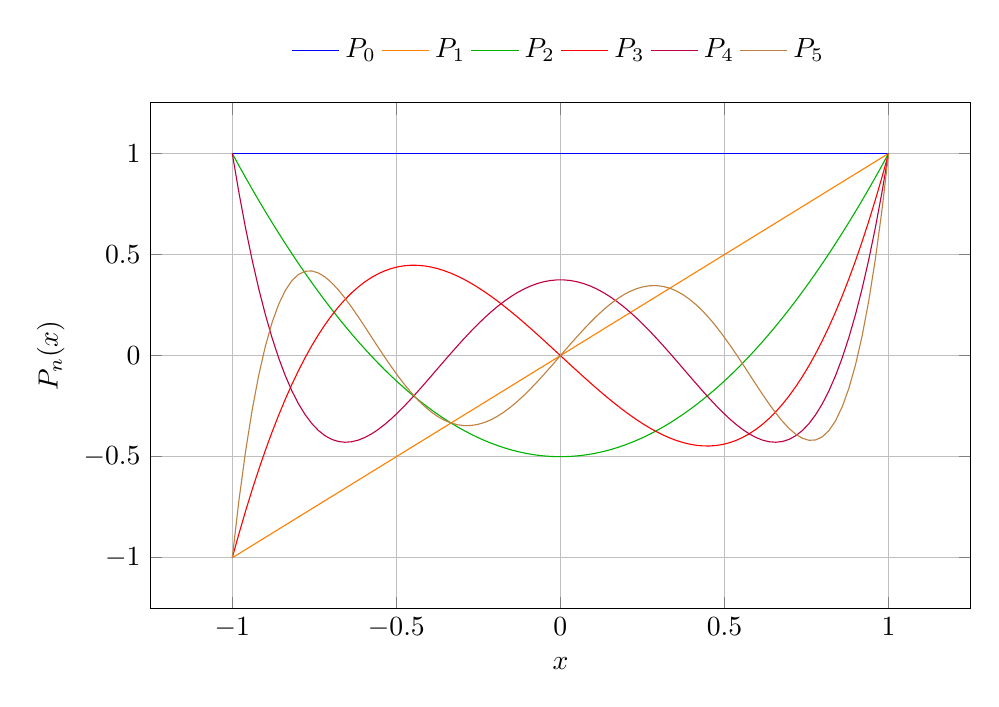
\begin{tikzpicture}
  \begin{axis}[
    width=12cm,
    height=8cm,
    xmin=-1.25, xmax=1.25,
    ymin=-1.25, ymax=1.25,
    xlabel={$x$}, ylabel={$P_n(x)$},
    xtick={-1,-0.5,0,0.5,1},
    ytick={-1,-0.5,0,0.5,1},
    grid=both,
    legend style={at={(0.5,1.15)},anchor=north,legend columns=6, fill=none, draw=none},
    legend cell align={left},
    samples=100
  ]
    % P_0(x) = 1
    \addplot[domain=-1:1, color=blue] {1};
    \addlegendentry{$P_0$}
    % P_1(x) = x
    \addplot[domain=-1:1, color=orange] {x};
    \addlegendentry{$P_1$}
    % P_2(x) = (3x^2-1)/2
    \addplot[domain=-1:1, color=green!70!black] {(3*x^2-1)/2};
    \addlegendentry{$P_2$}
    % P_3(x) = (5x^3-3x)/2
    \addplot[domain=-1:1, color=red] {(5*x^3-3*x)/2};
    \addlegendentry{$P_3$}
    % P_4(x) = (35x^4-30x^2+3)/8
    \addplot[domain=-1:1, color=purple] {(35*x^4-30*x^2+3)/8};
    \addlegendentry{$P_4$}
    % P_5(x) = (63x^5-70x^3+15x)/8
    \addplot[domain=-1:1, color=brown] {(63*x^5-70*x^3+15*x)/8};
    \addlegendentry{$P_5$}
  \end{axis}
\end{tikzpicture}
\end{document}
